\documentclass[a4paper,12pt]{article}
\usepackage[utf8x]{inputenc}
\usepackage{amssymb}
\usepackage{amsfonts}
\usepackage{mathrsfs}
\usepackage{amsmath}
\usepackage{amsthm}
\usepackage[margin=3cm]{geometry}
\usepackage{times}
\usepackage{graphicx}
\usepackage{enumitem}
\usepackage{fancyhdr}
\usepackage{hyperref}
\usepackage{setspace}
\usepackage{subcaption}
\usepackage{mathtools}

\pagestyle{fancy}
\fancyhf{}
\lhead{Thomas Delaney}
\rhead{Effect of time bin widths on correlations}
\cfoot{\thepage}

\newtheorem{theorem}{Theorem}
\newtheorem{proposition}{Proposition}[section]
\newtheorem{lemma}{Lemma}[section]
\newtheorem{corollary}{Corollary}[section]
\theoremstyle{definition}
\newtheorem{definition}{Definition}[section]

\newcommand{\boldnabla}{\mbox{\boldmath$\nabla$}} % to be used in mathmode
\newcommand{\cbar}{\overline{\mathbb{C}}}% to be used in mathmode
\newcommand{\diff}[2]{\frac{d #1}{d #2}}% to be used in mathmode
\newcommand{\difff}[2]{\frac{d^2 #1}{d #2^2}}% to be used in mathmode
\newcommand{\pdiff}[2]{\frac{\partial #1}{\partial #2}} % to be used in mathmode
\newcommand{\pdifff}[2]{\frac{\partial^2 #1}{\partial #2^2}}% to be used in mathmode
\newcommand{\upperth}{$^{\mbox{\footnotesize{th}}}$}%to be used in text mode
\newcommand{\vect}[1]{\mathbf{#1}}% to be used in mathmode
\newcommand{\curl}[1]{\boldnabla \times \vect{#1}} % to be used in mathmode
\newcommand{\divr}[1]{\boldnabla \cdot \vect{#1}} %to be used in mathmode
\newcommand{\modu}[1]{\left| #1 \right|} %to be used in mathmode
\newcommand{\brak}[1]{\left( #1 \right)} % to be used in mathmode
\newcommand{\comm}[2]{\left[ #1 , #2 \right]} %to be used in mathmode
\newcommand{\dop}{\vect{d}} %to be used in mathmode
\newcommand{\cov}{\text{cov}} %to be used in mathmode
\newcommand{\var}{\text{var}} %to be used in mathmode
\newcommand{\mb}{\mathbf} %to be used in mathmode
\newcommand{\bs}{\boldsymbol} %to be used in mathmode
% Title Page
\title{How informative are retinal ganglion cells?}
\author{Thomas Delaney 1330432}

\begin{document}

\tableofcontents

\newpage

\section{Motivation}
In their review entitled `Measuring and interpreting neural correlations', Cohen and Kohn studied the effects of response strength and time bin width on neural correlation measurement. Using simulated data, they found that correlation measurements taken between weakly responding neurons (i.e. neurons with firing rates of $<10$ spikes per s) will be less than the true pairwise correlation value. They also found that binning the neural spiking data into small time bins can cause the measured correlation to be less than the true value. How small is 'small' in this case is related to width of the cross-correlogram of the pair of neurons. But, it was shown in simulation that time bins should be at least $0.1$ seconds wide in order for the measured correlation value to be close to the true correlation value \cite{cohen}.

Our aim here is to measure a big enough sample of pairwise correlations from actual neural data across a selection of time bin widths and compare our results to those of Cohen and Kohn. In order to do this we used data collected using `Neuropixels' probes \cite{jun}. These data are made available publicly online by Dr. Nick Steinmetz \footnote{\url{http://data.cortexlab.net/dualPhase3/}}.

\section{Data}
The recent development of Neuropixels probes has allowed extracellular voltage measurements to be collected from multiple brain regions simultaneously routinely, and in much larger numbers than traditional methods.

Using two probes, spiking activity was simultaneously collected from over $800$ neurons in an awake mouse brain for a period of $84$ minutes. During this period, the mouse was shown various visual stimuli. The $800$ neurons were distributed across $5$ different brain regions: V1, hippocampus, thalamus, motor cortex, and striatum.

The data consist of spike timings and cell/cluster identifiers associating spikes with a certain cell/cluster and a certain time. Each cell/cluster is classified as `good', `multi-unit activity', or `unsorted', referring to the quality of spike sorting. This classification was performed by those who analysed the data. Only the cell/clusters classified as `good' are used in this project.

\subsection{Stimulus}

The stimulus was a full field moving bar grating. There were $17$ stimulus conditions corresponding to $16$ drift directions ($0$ degrees to $337.5$ degrees in $22.5$ degree increments) with $2$Hz temporal frequency and $0.08$ cycles/degree spatial frequency (conditions $1-16$) plus a blank condition ($17$). Each condition was presented $10$ times for $2$ seconds each time, with $1.5$ seconds between trials.

\section{Methods}
\subsection{Binning data}
The data were divided into time bins or various widths ranging from $0.01$ to $2$ seconds. If the bin width was not an integer divisor of the trial period ($2$ seconds), only the bins that lay totally within the trial period were included. For example, when dividing the trials into bins of $0.3$ seconds, the final bin of $0.2$ seconds was excluded. We measured the number of spikes in each time bin.

When performing calculations on the binned data, each bin was treated as an individual measurement. For example, when calculating the spike count correlation coefficient for a given pair of neurons, if the time bin used was $2.0$ seconds, then we had $10$ measurements for each neuron with which to calculate the coefficient. But, if we were using a bin width of $1.0$ second, then we would have $20$ measurements for each neuron.

\subsection{Pairing strongly responding neurons}
A weak response, or low firing rate, has a diminishing effect on measured correlation \cite{cohen}. In order to avoid this effect, we filtered out any neurons with a mean firing rate of less than $10$ spikes per second measured across the $10$ trials. Once these neurons were filtered out, we randomly chose $30$ pairs from all the possible pairs of the remaining neurons. We used these $30$ pairs to calculate $30$ correlation coefficients. We repeated this process for each brain region, and each stimulus condition.

If less than $9$ strongly responding neurons were found it was not possible to make $30$ pairs of strongly responding neurons. In that case, we just used all the strongly responding pairs.

\subsection{Correlation coefficients}
We calculated Pearson's correlation coefficient for pairs of neurons. For jointly distributed random variables $X$ and $Y$, Pearson's correlation coefficient is defined as:
\begin{align}\label{eq:dist_pearsons_corr}
  \rho_{XY} =& \frac{\cov(X,Y)}{\sigma_X \sigma_Y} \\
            =& \frac{E[(X - \mu_X)(Y - \mu_Y)]}{\sigma_X \sigma_Y}
\end{align}
where $E$ denotes the expected value, $\mu$ denotes the mean, and $\sigma$ denotes the standard deviation. The correlation coefficient is a normalised measure of the covariance. It can take values between $1$ (completely correlated) and $-1$ (completely anti-correlated). Two independent variables will have a correlation coefficient of $0$. But, having $0$ correlation does not imply independence.

If we do not know the means and standard deviations required for equation \ref{eq:dist_pearsons_corr}, but we have samples from $X$ and $Y$, Pearson's sample correlation coefficient is defined as:
\begin{align}
  r_{XY} = \frac{\sum_{i=1}^n (x_i - \bar{x})(y_i - \bar{y})}{\sqrt{\sum_{i=1}^n (x_i - \bar{x})^2}\sqrt{\sum_{i=1}^n (y_i - \bar{y})^2}}
\end{align}
where $\lbrace (x_i, y_i) \rbrace$ for $i \in \lbrace 1, \dots, n \rbrace$ are the paired samples from $X$ and $Y$, and $\bar{x} = \frac{1}{n}\sum_{i=1}^n x_i$, and $\bar{y} = \frac{1}{n}\sum_{i=1}^n y_i$ are the sample means.

In practice we used the python function \texttt{scipy.stats.pearsonr} to calculate the correlation coefficients.

\subsubsection{Spike Count Correlation, $r_{SC}$}
The spike count correlation ($r_{SC}$) of two cells is the correlation between the spike counts of those cells in response to a given stimulus condition.

\subsubsection{Signal Correlation, $r_{signal}$}
The signal correlation of two cells ($r_{signal}$) is the correlation between the mean responses of those cells to each stimulus condition.

\subsubsection{Separating Correlations \& Anti-correlations}\label{sec:corr_anti_corr}
In order to compare the effect of bin width on measures of negative $r_{SC}$ (anti-correlation) and positive $r_{SC}$ separately, we had to separate correlated and anti-correlated pairs. To do this, we simply measured the mean $r_{SC}$, taking the mean across all the bin widths. If this quantity was positive or zero we regarded the pair as positively correlated. If this quantity was negative we regarded the pair as anti-correlated.

\subsection{Mutual Information}
\subsubsection{Entropy $H(X)$}
The entropy of a random variable $X$, with outcomes $x_1, \dots, x_N$, and corresponding probabilities $p_1, \dots, p_N$ is defined as
\begin{align}\label{entropy}
H(X) = -\sum_{n=1}^N p_n \log _2 p_n
\end{align}
This quantity is also known as the information entropy or the `surprise'. It measures the amount of uncertainty in a random variable. For example, a variable with a probability of $1$ for one outcome, and zero for all other outcomes will have 0 entropy, because it contains no uncertainty. But a variable with a uniform distribution will have maximal entropy as it is the least predictable. This quantity is analogous to the entropy of a physical system \cite{shannon}. Note that any base may be used for the logarithm in equation \ref{entropy}, but using base $2$ means that the quantity will be measured in `bits'.

The joint entropy of two jointly distributed random variables $X$ and $Y$, where $Y$ has outcomes $y_1, \dots, y_M$, is defined as
\begin{align}\label{joint_entropy}
H(X, Y) = -\sum_{n=1}^N \sum_{m=1}^M P(X=x_n, Y=y_m) \log _2 P(X=x_n, Y=y_m)
\end{align}
If $X$ and $Y$ are independent then $H(X,Y) = H(X) + H(Y)$. Otherwise $H(X,Y) \leq H(X) + H(Y)$. When $X$ and $Y$ and completely dependent $H(X,Y) = H(X) = H(Y)$.

The conditional entropy of $Y$ conditioned on $X$ is defined as
\begin{align}
H(Y|X) = -\sum_{n=1}^N \sum_{m=1}^M P(X=x_n, Y=y_m) \log _2 \frac{P(X=x_n, Y=y_m)}{P(X=x_n)}
\end{align}
When $X$ and $Y$ are independent $H(Y|X) = H(Y)$. Intuitively, we learn nothing of $Y$ by knowing $X$, so $Y$ is equally uncertain whether we know $X$ or not. If $Y$ is totally dependent on $X$, then the fraction in the logarithm is $1$, which gives $H(Y|X) = 0$.

These entropy measures are the basis of the mutual information measure.

\subsubsection{Mutual Information $I(X;Y)$}
The mutual information can be defined mathematically in a number of ways, all of which are equivalent. For two jointly distributed random variables $X$ and $Y$, the mutual information $I(X;Y)$ is defined as
\begin{align}\label{eq:mutual_info_intuitive}
I(X;Y)  =& H(Y) - H(Y|X) \\
        =& H(X) - H(X|Y)
\end{align}
Equation \ref{eq:mutual_info_intuitive} fits with the following intuition: The mutual information between $X$ and $Y$ is the reduction in uncertainty about $X$ gained by knowing $Y$, or vice versa. We could also say the mutual information is the amount of information gained about $X$ by knowing $Y$, or vice versa.

Another useful entropy based definition for the mutual information is
\begin{align}
I(X;Y)  =& H(X) + H(Y) - H(X,Y)
\end{align}
This definition is useful because it does not require the calculation of conditional probabilities. This was the form we used when performing calculations.

The mutual information can also be defined in terms of marginal, joint, and conditional distributions. For example,
\begin{align}
I(X;Y)  =& -\sum_{n=1}^N \sum_{m=1}^M P(X=x_n, Y=y_m) \log _2 \frac{P(X=x_n, Y=y_m)}{P(X=x_n) P(Y=y_m)}
\end{align}
Notice that this can be rewritten as a Kullback–Leibler divergence.
\begin{align}
I(X;Y)  =& D_{KL}(P(X,Y)|| P(X)P(Y))
\end{align}
So, we can also think of the mutual information as a measure of the difference between the joint distribution of $X$ and $Y$, and the product of their marginal distributions. Since the product of the marginal distributions is the joint distribution for independent variables. We can further think of the mutual information as a measure of the variables' dependence on one another.

\section{Results}
\subsection{Varying bin width}
In order to investigate the effect of bin width on the various measures we used, we took these measurements using a number of different values for the bin width. We found that the bin width definitely had an effect on the spike count correlation, and the mutual information.

\subsubsection{Spike count correlations at various bin widths}
For each stimulus condition and each region, we randomly chose $30$ pairs of strongly responding neurons (or chose as many pairs as we could find), measured their absolute spike count correlations ($|r_{SC}|$) and absolute signal correlation ($|r_{signal}|$) using various values for the time bin width and examined the relationship between the coefficients and the bin width. We found that $|r_{SC}|$ increased approximately log-linearly up to a width of $1$s and appeared to level off thereafter, see figure \ref{fig:bin_width_vs_correlation_by_region}, or figure \ref{fig:linear_bin_width_vs_correlation_by_region} for a linear version. This is in agreement with the findings of the simulated experiment in \cite{cohen}. For these figures, we chose the stimulus condition that evoked the strongest response from a given region. This guaranteed us $30$ strongly responding pairs for each region.

\subsubsection{Correlations \& Anti-correlations}
We separated the $30$ randomly chosen pairs into correlated and anti-correlated pairs as per section \ref{sec:corr_anti_corr}. We then measured $r_{SC}$ across various bin width values. We found that the positive $r_{SC}$ got more positive as the bin width increased. We also found that the negative $r_{SC}$ got more negative as the bin width increased. Both positive and negative coefficients showed a log-linear increase similar to the absolute spike count correlation coefficients. See figure \ref{fig:corr_anti_corr_by_region}.

\subsubsection{Signal Correlations}
We found that $|r_{signal}|$ maintained a constant value across different bin widths. This was the case in all regions, with some variations in V1. See figure \ref{fig:linear_bin_width_vs_signal_correlation_by_region}.

\subsubsection{Mutual Information}

\subsection{Spike count correlation \& Mutual Information distributions}
\subsubsection{Spike count correlation histograms}
For each region, we found all of the cells that responded to the stimulus. We randomly selected $1000$ pairs from all possible pairs of these cells, and we measured their pairwise  spike count correlations. We created histograms using these data in order to examine the distributions of $|r_{SC}|$ in each region, see figure \ref{fig:all_corr_histograms}.

\begin{figure}[p]
  \begin{subfigure}{0.5\textwidth}
    \centering
    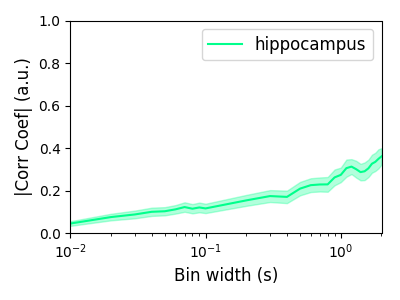
\includegraphics[width=\textwidth]{figures/bin_width_correlations_hippocampus_15.png}
  \end{subfigure}
  \begin{subfigure}{0.5\textwidth}
    \centering
    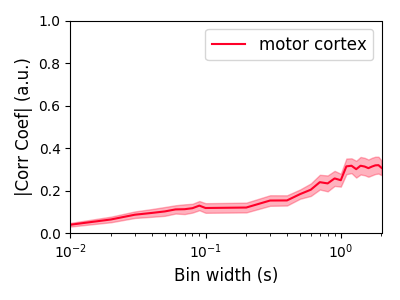
\includegraphics[width=\textwidth]{figures/bin_width_correlations_motor_cortex_15.png}
  \end{subfigure}
  \begin{subfigure}{0.5\textwidth}
    \centering
    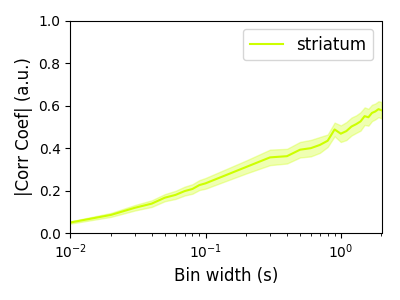
\includegraphics[width=\textwidth]{figures/bin_width_correlations_striatum_14.png}
  \end{subfigure}
  \begin{subfigure}{0.5\textwidth}
    \centering
    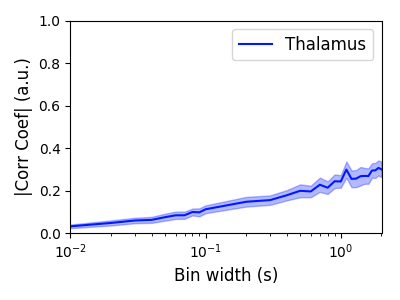
\includegraphics[width=\textwidth]{figures/bin_width_correlations_thalamus_15.png}
  \end{subfigure}
  \begin{subfigure}{0.5\textwidth}
    \centering
    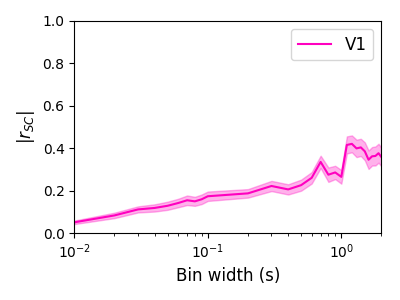
\includegraphics[width=\textwidth]{figures/bin_width_correlations_v1_6.png}
  \end{subfigure}
  \caption{\textbf{Spike Count Correlations:} Absolute values of correlation coefficients measured using different time bin widths. Shaded areas indicate standard errors. One figure for each brain region from which data were available. The absolute correlation increases approximately log-linearly with the bin width up to a bin width of $1$ second and levels out somewhat thereafter.}
  \label{fig:bin_width_vs_correlation_by_region}
\end{figure}

\begin{figure}[p]
  \begin{subfigure}{0.5\textwidth}
    \centering
    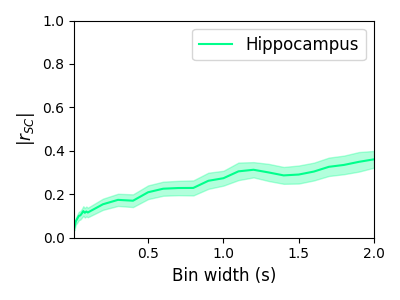
\includegraphics[width=\textwidth]{figures/linear_bin_width_correlations_hippocampus_15.png}
  \end{subfigure}
  \begin{subfigure}{0.5\textwidth}
    \centering
    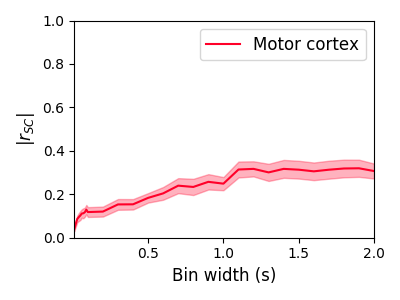
\includegraphics[width=\textwidth]{figures/linear_bin_width_correlations_motor_cortex_15.png}
  \end{subfigure}
  \begin{subfigure}{0.5\textwidth}
    \centering
    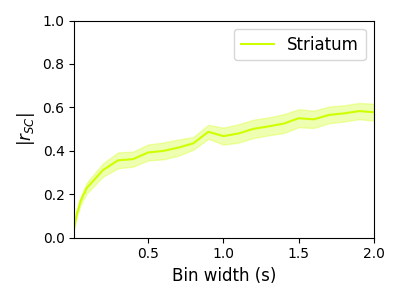
\includegraphics[width=\textwidth]{figures/linear_bin_width_correlations_striatum_14.png}
  \end{subfigure}
  \begin{subfigure}{0.5\textwidth}
    \centering
    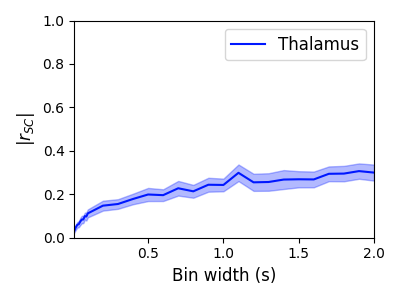
\includegraphics[width=\textwidth]{figures/linear_bin_width_correlations_thalamus_15.png}
  \end{subfigure}
  \begin{subfigure}{0.5\textwidth}
    \centering
    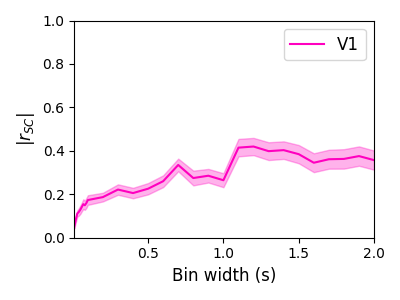
\includegraphics[width=\textwidth]{figures/linear_bin_width_correlations_v1_6.png}
  \end{subfigure}
  \caption{\textbf{Spike Count Correlations:} Absolute values of correlation coefficients measured using different time bin widths. Shaded areas indicate standard errors. One figure for each brain region from which data were available. The absolute correlation increases approximately log-linearly with the bin width up to a bin width of $1$ second and levels out somewhat thereafter.}
  \label{fig:linear_bin_width_vs_correlation_by_region}
\end{figure}

\begin{figure}[p]
  \begin{subfigure}{0.5\textwidth}
    \centering
    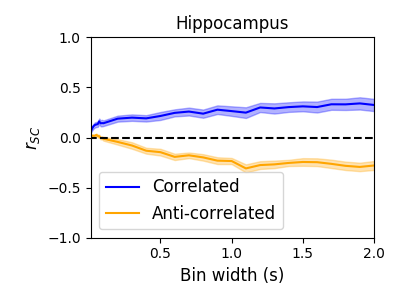
\includegraphics[width=\textwidth]{figures/linear_bin_width_relative_correlations_hippocampus_15.png}
  \end{subfigure}
  \begin{subfigure}{0.5\textwidth}
    \centering
    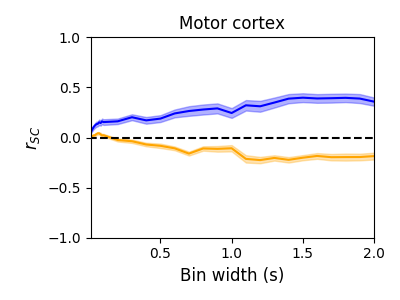
\includegraphics[width=\textwidth]{figures/linear_bin_width_relative_correlations_motor_cortex_15.png}
  \end{subfigure}
  \begin{subfigure}{0.5\textwidth}
    \centering
    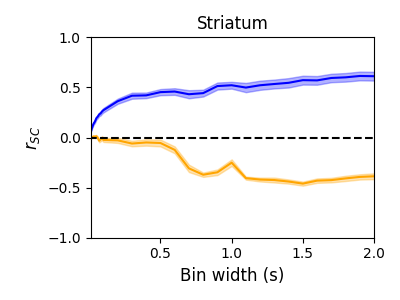
\includegraphics[width=\textwidth]{figures/linear_bin_width_relative_correlations_striatum_14.png}
  \end{subfigure}
  \begin{subfigure}{0.5\textwidth}
    \centering
    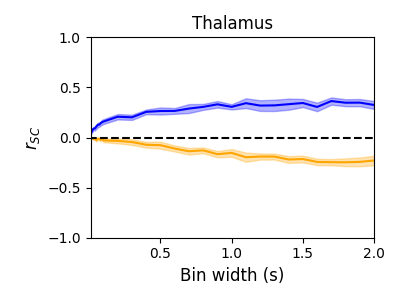
\includegraphics[width=\textwidth]{figures/linear_bin_width_relative_correlations_thalamus_15.png}
  \end{subfigure}
  \begin{subfigure}{0.5\textwidth}
    \centering
    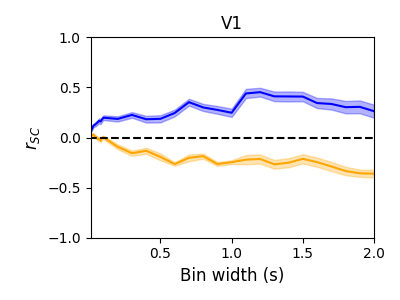
\includegraphics[width=\textwidth]{figures/linear_bin_width_relative_correlations_v1_6.png}
  \end{subfigure}
  \caption{\textbf{Spike Count Correlations and Anti-correlations:} Correlation coefficients measured using different time bin widths and separated into positive and negative sets. Shaded areas indicate standard errors. One figure for each brain region from which data were available. The correlations or anti-correlations get stronger as the bin width increases. We see the log linear increase similar to figures \ref{fig:bin_width_vs_correlation_by_region} and \ref{fig:linear_bin_width_vs_correlation_by_region}.}
  \label{fig:corr_anti_corr_by_region}
\end{figure}

\begin{figure}[p]
  \begin{subfigure}{0.5\textwidth}
    \centering
    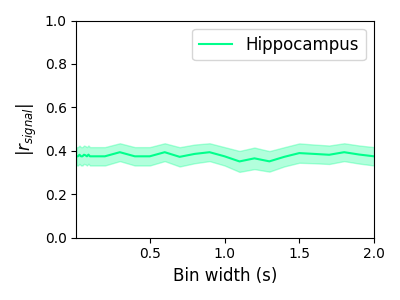
\includegraphics[width=\textwidth]{figures/signal_linear_bin_width_correlations_hippocampus_0.png}
  \end{subfigure}
  \begin{subfigure}{0.5\textwidth}
    \centering
    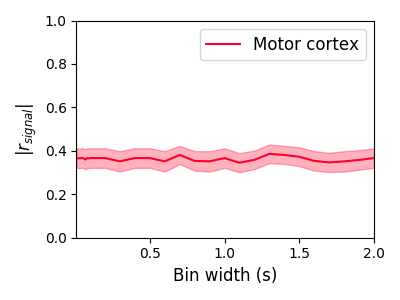
\includegraphics[width=\textwidth]{figures/signal_linear_bin_width_correlations_motor_cortex_0.png}
  \end{subfigure}
  \begin{subfigure}{0.5\textwidth}
    \centering
    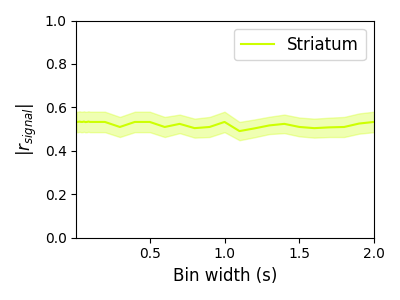
\includegraphics[width=\textwidth]{figures/signal_linear_bin_width_correlations_striatum_0.png}
  \end{subfigure}
  \begin{subfigure}{0.5\textwidth}
    \centering
    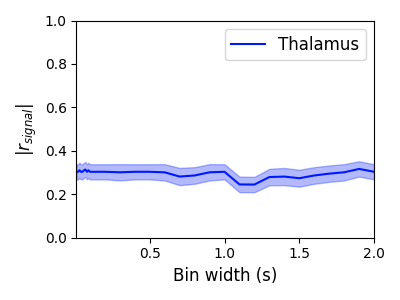
\includegraphics[width=\textwidth]{figures/signal_linear_bin_width_correlations_thalamus_0.png}
  \end{subfigure}
  \begin{subfigure}{0.5\textwidth}
    \centering
    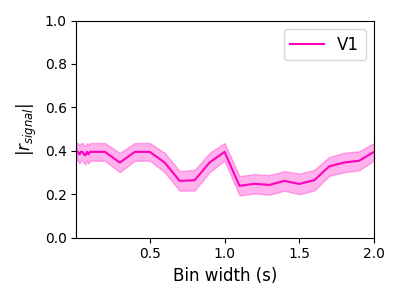
\includegraphics[width=\textwidth]{figures/signal_linear_bin_width_correlations_v1_0.png}
  \end{subfigure}
  \caption{\textbf{Signal Correlations:} Absolute values of signal correlation coefficients measured using different time bin widths. Shaded areas indicate standard errors. One figure for each brain region from which data were available. The signal correlation maintains a fairly constant value across bin widths for most brain regions, with some variations in V1.}
  \label{fig:linear_bin_width_vs_signal_correlation_by_region}
\end{figure}

\begin{figure}[p]
  \begin{subfigure}{0.5\textwidth}
    \centering
    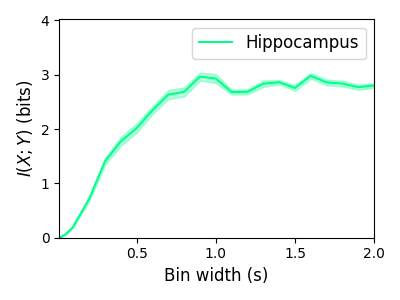
\includegraphics[width=\textwidth]{figures/linear_mutual_info_by_bin_width_hippocampus_15.png}
  \end{subfigure}
  \begin{subfigure}{0.5\textwidth}
    \centering
    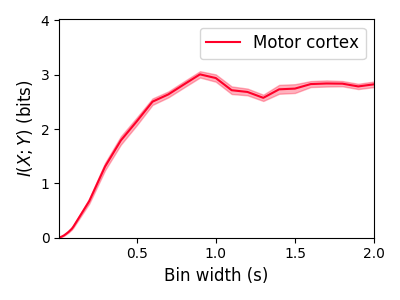
\includegraphics[width=\textwidth]{figures/linear_mutual_info_by_bin_width_motor_cortex_15.png}
  \end{subfigure}
  \begin{subfigure}{0.5\textwidth}
    \centering
    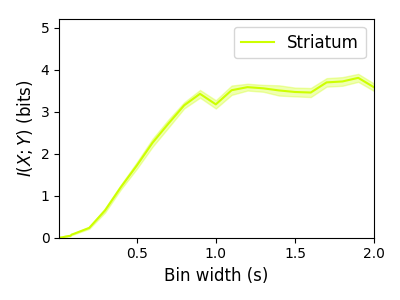
\includegraphics[width=\textwidth]{figures/linear_mutual_info_by_bin_width_striatum_14.png}
  \end{subfigure}
  \begin{subfigure}{0.5\textwidth}
    \centering
    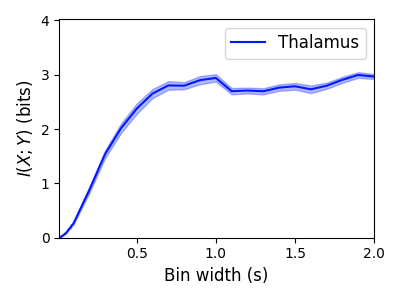
\includegraphics[width=\textwidth]{figures/linear_mutual_info_by_bin_width_thalamus_15.png}
  \end{subfigure}
  \begin{subfigure}{0.5\textwidth}
    \centering
    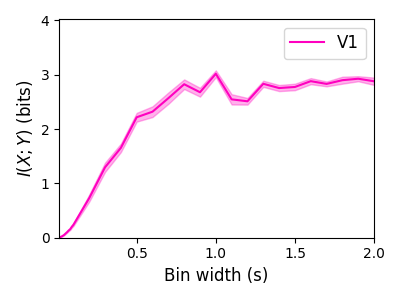
\includegraphics[width=\textwidth]{figures/linear_mutual_info_by_bin_width_v1_6.png}
  \end{subfigure}
  \caption{\textbf{Mutual Information:} Mutual information measured using different time bin widths. Shaded areas indicate standard errors. One figure for each brain region from which data were available. The mutual information increases as the the bin width increases, reaching a limit of about $3$ bits for bin widths $\geq 1$s.}
  \label{fig:linear_bin_width_vs_mutual_information_by_region}
\end{figure}

\begin{figure}[p]
  \begin{subfigure}{0.5\textwidth}
    \centering
    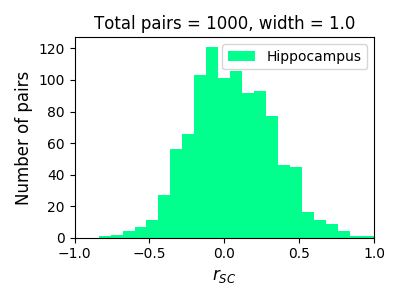
\includegraphics[width=\textwidth]{figures/all_hippocampus_8_1p0_correlation_histogram.png}
  \end{subfigure}
  \begin{subfigure}{0.5\textwidth}
    \centering
    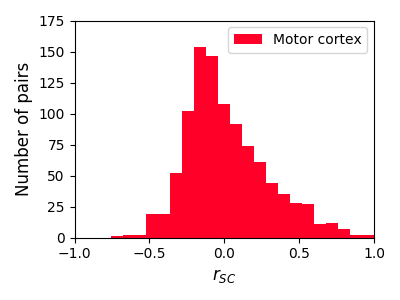
\includegraphics[width=\textwidth]{figures/all_motor_cortex_8_1p0_correlation_histogram.png}
  \end{subfigure}
  \begin{subfigure}{0.5\textwidth}
    \centering
    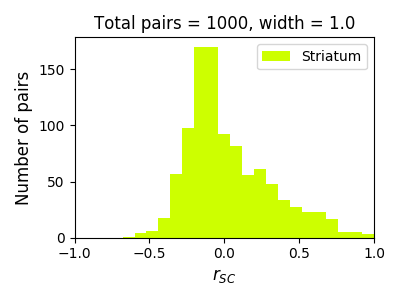
\includegraphics[width=\textwidth]{figures/all_striatum_8_1p0_correlation_histogram.png}
  \end{subfigure}
  \begin{subfigure}{0.5\textwidth}
    \centering
    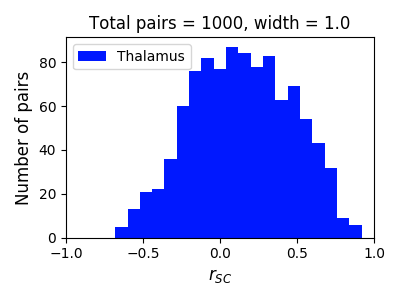
\includegraphics[width=\textwidth]{figures/all_thalamus_8_1p0_correlation_histogram.png}
  \end{subfigure}
  \begin{subfigure}{0.5\textwidth}
    \centering
    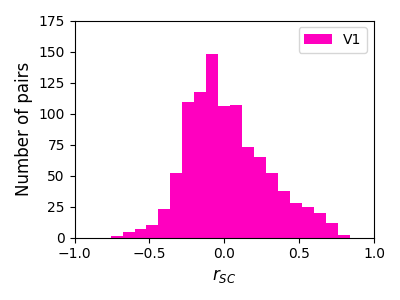
\includegraphics[width=\textwidth]{figures/all_v1_8_1p0_correlation_histogram.png}
  \end{subfigure}
  \caption{\textbf{Spike Count Correlation Histograms:} Histograms of the spike count correlations of $1000$ randomly chosen pairs of neurons from within each region. The motor cortex, V1, and striatum all have similar distributions. For these regions the mean $r_{SC}$ is positive, but the median $r_{SC}$ is negative, so their distributions are skewed. The hippocampus is slightly different in that both the median and the mean are positive but close to $0$. The thalamus is different to all the other regions. Both its mean and medium are positive and are aprroximately equal to $0.14$.}
  \label{fig:all_corr_histograms}
\end{figure}

\section*{Things to discuss with Cian}
\begin{enumerate}
  \item Is all of the above clear?
  \item Are my methods sound?
  \item Could any of my methods be improved?
  \item How can this document be improved? (The figures with the linear x-axis might be better.)
\end{enumerate}


\newpage

\bibliography{fluorescence_modelling.bbl}

\end{document}
